\RequirePackage[OT1]{fontenc}
\documentclass[conference]{IEEEtran}
\usepackage{cite,amsmath,amssymb,amsfonts,graphicx,balance,url,algorithmic,algorithm}
\renewcommand{\algorithmicrequire}{\textbf{Input:}}
\renewcommand{\algorithmicensure}{\textbf{Output:}}
\usepackage[hidelinks]{hyperref}
\newcommand{\ind}{\mathbf{1}}
\begin{document}
\title{Evaluating Verified-Support Gating in Two-Model Adaptive Intrusion Detection}
\author{
\IEEEauthorblockN{Gilang Wasis Wicaksono\textsuperscript{*}}
\IEEEauthorblockA{\textit{School of Computing}\\
\textit{Telkom University}\\
Bandung, Indonesia\\
gilangwasis@student.telkomuniversity.ac.id}
\and
\IEEEauthorblockN{Vera Suryani}
\IEEEauthorblockA{\textit{School of Computing}\\
\textit{Telkom University}\\
Bandung, Indonesia\\
verasuryani@telkomuniversity.ac.id}}
\maketitle
\begin{abstract}
We evaluate verified-support gating (GDT) in adaptive intrusion detection using histogram gradient boosting, weighted seven-nearest neighbors, a correction ledger, and separate threshold audits. After 480 development and 390 original confirmation runs, a frozen extension compared native adaptive random forests on two unused 12,000-flow captures with matched 5\% label acquisition. GDT achieved 96.46\%/91.45\% balanced accuracy on Hulk/DDoS, versus 89.10\%/78.08\% for native ARF. Incremental gate gains over verified-only were 0.29/0.55 percentage points. Neither new capture met the one-point incremental target. Contributions are controlled integration and post-feedback opportunity analysis. All annotations were simulated; human effectiveness remains unmeasured.
\end{abstract}
\begin{IEEEkeywords}
intrusion detection, adaptive learning, delayed feedback, local support, controlled evaluation
\end{IEEEkeywords}

\section{Introduction}
Changing traffic can degrade historically trained detectors. Adaptive learning uses new evidence but is distinct from drift detection~\cite{gama,lu}. Attack labels can be scarce, delayed, or corrected after use. Feature/label corrections in CICIDS2017~\cite{sharaf,engelen,liu} and risks of security-evaluation bias~\cite{arp,tesseract} indicate that score improvements must be interpreted alongside data provenance and temporal order.

The research problem is \emph{benefit attribution}: gains from combining two models, retraining, and threshold adjustment do not identify which component helps. Incremental gate benefit requires controls with the same labels and update schedule. Labels arriving after an attack burst can also update a model without leaving similar attacks on which to test its benefit. Evaluation therefore connects decisions to available feedback and post-fit prediction opportunities.

We ask: \textbf{RQ1}, does updating improve balanced accuracy (BA) over frozen detection while preserving source retention and low false-positive rate (FPR)? \textbf{RQ2}, does gating improve on verified-only/simple-maximum controls under matched feedback? \textbf{RQ3}, how do delay, corrections, and remaining post-fit attacks limit adaptation?

The objectives are to measure adaptive-package benefit (RQ1), isolate the incremental gate path (RQ2), and explain limitations from feedback timing/availability (RQ3). Histogram gradient boosting (HGB) detects nonlinear patterns; nearest neighbors provide traceable local support. This separation enables decision-path testing with shared learning trajectories.

Contributions are (1) a feedback contract with revisions and separate audits; (2) matched-acquisition gate/controller controls; and (3) 870 original audited runs, ARF with shared queries, and two additional captures with post-fit opportunity analysis. The main contribution is controlled evaluation of this integration; HGB and nearest neighbors are established components, and gate superiority remains a hypothesis to test.

\section{Related Work}
\subsection{Streaming Adaptation and Memory}
Paired Learners replaces a stable learner using error differences from a reactive learner~\cite{paired}; SAM-kNN adapts concept memory~\cite{sam}. ADWIN adjusts windows~\cite{adwin}, while adaptive random forests (ARF) use adaptive ensembles and have evaluated delayed labels~\cite{arf}. We isolate local-support gating with fixed refit schedules; two models or delayed feedback alone is not novel.

\subsection{Second Models and Label Acquisition}
SOUL combines memory replay/projection with high-confidence labels~\cite{soul}; SSF selects drift patterns and forgets obsolete memory~\cite{ssf}. ML2 instead scores flows and selects requests without generating training targets. Verified-only retains its acquisition to isolate the additional decision path.

\subsection{Delayed Feedback and Label Quality}
Jeon--Kim connects recovery to the diversity of arriving samples~\cite{jeon}; NAFN addresses noise in few-shot incremental learning~\cite{nafn}; ACORN-IDS learns novelty from normal data~\cite{acorn}. We track revisions and post-fit attacks to assess learning opportunities (Table~\ref{tab:lit}); ARF is rerun below; other studies provide context.

\begin{table*}[t]
\caption{Prior approaches and the contribution evaluated in this study}
\label{tab:lit}\centering\footnotesize
\begin{tabular}{p{.17\textwidth}p{.33\textwidth}p{.40\textwidth}}
\hline
Study / RQ & Prior focus & Specific distinction and evaluated contribution \\\hline
Paired Learners~\cite{paired}; SAM-kNN~\cite{sam} / RQ1--2 & Stable--reactive learner replacement; concept memory. & HGB detection and NN local scoring; incremental decision path tested under matched acquisition.\\
ADWIN~\cite{adwin}; ARF~\cite{arf} / RQ1,3 & Adaptive windows/ensembles; ARF evaluates delays. & Native ARF rerun with shared acquisition; refit/revision rules are explicit.\\
SOUL~\cite{soul} / RQ1--2 & Replay, memory projection, and label generation. & No pseudo-label training; training and audit labels are separate.\\
SSF~\cite{ssf} / RQ1--2 & Drift selection and strategic forgetting. & Fixed source replay/recent windows; disjoint retention probes and a maximum control.\\
Jeon--Kim~\cite{jeon} / RQ3 & Recalibration, buffered few-shot learning, and arrival bias. & Counts attacks after a correct label enters an ML1/ML2 fit.\\
NAFN~\cite{nafn} / RQ2--3 & Denoising and few-shot class-incremental learning. & Binary targets with delay/revisions; no claim of matching 50\% noise tolerance.\\
ACORN-IDS~\cite{acorn} / RQ1,3 & Continual novelty detection from normal data. & Measures dependence on positive labels and failure on rare attacks.\\\hline
\noalign{\vskip 2pt}
\textbf{This study / RQ1--3} & \textbf{Frozen HGB--7-NN integration, separate audits, and a correction ledger.} & \textbf{ARF with shared queries and two new captures; gate gains 0.29/0.55 BA points on Hulk/DDoS.}\\[2pt]\hline
\end{tabular}
\end{table*}

\section{Method and System Implementation}
\subsection{Stream Specification and Closed-Loop Architecture}
Fig.~\ref{fig:architecture} separates input streams, processing, and outputs. ML1 detects attacks; ML2 provides local support; audit labels adjust thresholds. For corrected CIC confirmation, inputs $x_i\in\mathbb R^{82}$ exclude labels, IP addresses, ports, identifiers, and timestamps to avoid testbed shortcuts~\cite{arp}. Median imputation handles missing values, signed-log transformation reduces tails, standardization aligns distance scales, and clipping to $[-10,10]$ limits extremes. All transformations are fitted only on historical BASE data. Freezing them makes outcome changes easier to attribute to model updates rather than to changes in feature space derived from test captures.

For flow $i$, $a_i$ denotes feedback availability, $h_i=1$ marks audit allocation, and $\tilde y_i(t)$ is its latest arrived label revision:
\begin{align}
 V_t&=\{(i,\tilde y_i(t)):a_i\le t,\ h_i=0\},\nonumber\\
 A_t&=\{(i,\tilde y_i(t)):a_i\le t,\ h_i=1\},\quad V_t\cap A_t=\varnothing.\label{eq:ledger}
\end{align}
The ledger records timing/revisions. Audits never train classifiers; corrections replace targets without rewriting predictions. This separation limits using the same label for classifier fitting and threshold selection, while stored predictions preserve evaluation according to knowledge available at issuance. A reused audit window is not an independent test set.

\begin{figure*}[t]
\centering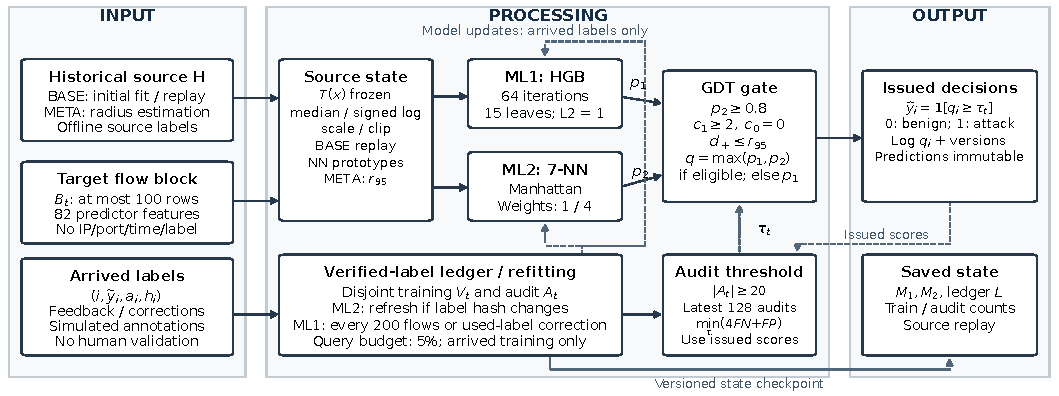
\includegraphics[width=.98\textwidth]{figures/architecture_ipo.pdf}
\caption{Input--processing--output architecture. Solid arrows carry data/state; dashed arrows carry model or threshold feedback and issued audit scores. Historical source state is fixed; only arrived training labels update classifiers. Audit labels tune the threshold using stored scores. Predictions are immutable. Source clustering supports query diversity, not a third classifier.}
\label{fig:architecture}
\end{figure*}

\subsection{Primary Detector and Replay Memory}
Gradient boosting captures nonlinear interactions~\cite{friedman}; HGB bins candidate splits, drawing on LightGBM~\cite{lightgbm,sklearn}. Development compared HGB/ExtraTrees under retention/FPR constraints. Selected HGB uses 64 iterations, rate 0.1, 15 leaves, 64 bins, minimum 20 samples/leaf, $L_2=1$, and no early stopping to preserve explicit cadence. This detector supports testing tabular feature interactions through periodic refitting; binning limits candidate splits. Its selection does not establish HGB as the most accurate or fastest option for every stream.

Initial fitting uses at most 8,192 BASE samples. Subsequent fits combine a fixed source replay set $S$ of at most 1,024 samples (at most 512 per class, without replacement) and up to 1,024 recent arrived training labels:
\begin{align}
 D_t&=S\cup\operatorname{tail}_{1024}(V_t),\nonumber\\
 J_t(f)&=\sum_{i\in D_t}w_i\ell(\tilde y_i,f(x_i))+\Omega_{L_2}(f),\label{eq:loss}\\
 \ell(y,p)&=-y\log p-(1-y)\log(1-p).\nonumber
\end{align}
Replay preserves old examples, recent windows enable adaptation, and regularization limits complexity. Replay/prototype sets actually contain 684--706 source samples across seeds; class caps do not guarantee class balance. Source weights are 1; new-label weights $w_i=4\cdot2^{\tilde y_i}$ emphasize recent/attack evidence. Window caps control fit size, not total ledger storage; multiplier 2 was development-selected. Refit every 200 flows matches controls; used-target corrections trigger the next 100-flow boundary. Optimality is unproven~\cite{adwin,arf}.

\subsection{Local Scorer and Support Gate}
Nearest neighbors provide traceable evidence~\cite{cover,dudani}. ML2 uses seven Manhattan neighbors from up to 1,024 class-capped source prototypes and up to 1,024 recent verified examples, weighted $\omega_j=1$ and 4. Manhattan measures scaled absolute deviations; $k=7$ balances smoothing/locality without exhaustive optimization. For $d_j=\|x-x_j\|_1$:
\begin{equation}
 p_{2,t}(x)=\frac{\sum_{j\in\mathcal N_7(x)}\omega_j\tilde y_j/\max(d_j,10^{-6})}{\sum_{j\in\mathcal N_7(x)}\omega_j/\max(d_j,10^{-6})}.\label{eq:knn}
\end{equation}
The distance floor handles coincident examples. At block boundaries, changed training identities/labels refresh the index. Excluding pseudo-labels avoids self-reinforcing training.

Let $c_1,c_0$ count distinct recent feature hashes per class among the neighbors, and $d_+$ be the nearest recent positive distance. Let $r$ be the historical META 95th-percentile distance to initial prototypes:
\begin{align}
 g_t(x)&=\ind[p_{2,t}\ge0.8,\ c_1\ge2,\ c_0=0,\ d_+\le r],\label{eq:gate}\\
 q_t(x)&=p_{1,t}(x)+g_t(x)\max(0,p_{2,t}(x)-p_{1,t}(x)).\label{eq:raw}
\end{align}
High confidence filters weak support; two positive hashes limit dependence on a single example; excluding benign neighbors rejects local conflicts; the radius limits distant support. Hashes remove duplicates without establishing independence. The radius uses historical META data to avoid selection from test-capture labels. Strict conditions can reduce alarms while missing opportunities to rescue attacks. These frozen conservative heuristics require benefit/coverage evaluation; their thresholds are not theoretical optima.

\subsection{Audit Acquisition and Update Cycle}
After at least 20 audit labels arrive, up to the 128 latest audits by flow index select $\tau_t\in\{0.1,\ldots,0.9\}$:
\begin{equation}
 \tau_t=\arg\min_\tau\{4\operatorname{FN}(A_t,q,\tau)+\operatorname{FP}(A_t,q,\tau)\}.\label{eq:threshold}
\end{equation}
Raw $q_i$ is stored as \texttt{raw}; decision score $s_i$ as \texttt{p}. For the issued threshold $\tau_i$:
\begin{align}
 u_i&=\operatorname{clip}(q_i,10^{-10},1-10^{-10}),\nonumber\\
 s_i&=\frac{u_i(1-\tau_i)}{u_i(1-\tau_i)+(1-u_i)\tau_i}.\label{eq:issued}
\end{align}
Thus $s_i\ge0.5$ implements $q_i\ge\tau_i$. AP uses $s_i$ for systems and $p_{1,i}$/$p_{2,i}$ for raw models. Varying thresholds can change cross-block rankings.

Decisions $\hat y_t=\ind[q_t\ge\tau_t]$ use the raw score recorded at issuance; threshold ties favor proximity to 0.5, then lower cuts. Windows/minimums limit stale/sparse-label tuning without ensuring representativeness. The assumed 4:1 miss/alarm cost is not measured incident cost. Odds-shifted decision scores are not calibrated posteriors~\cite{guo}.

Active learning targets information~\cite{settles}. Per 100 flows, request one uniform audit, two uniform training samples, one ML2-uncertainty sample, and one distance-novelty sample preferring distinct clusters. Uniform sampling explores; uncertainty targets ambiguity; novelty/eight clusters promote diversity. Budget is 5\% (4\% training, 1\% audit): $B=5k$ for $N=100k$, with partial-block rounding. Settings are not proven optimal. Uniform audits are used so that threshold selection need not rely exclusively on flows that ML2 finds informative. Mixed requests allocate some budget to exploration and some to local information; the benefit of each part has not been isolated through ablation.

\begin{algorithm}[t]
\caption{GDT with delayed and revised feedback}
\label{alg:gdt}
\footnotesize
\begin{algorithmic}[1]
\REQUIRE History $H$, seed $s$, parameters $\theta$, blocks $\mathcal B$, queue $E$.
\ENSURE Issued predictions $P$, models $M_1,M_2$, ledger $L$.
\STATE $(M_1,M_2,r)\gets\operatorname{Init}(H,s,\theta)$.
\STATE $V,A,P,L,U_1\gets\varnothing$; $\tau\gets0.5$; $h_2\gets\bot$.
\FOR{each $B\in\mathcal B$ in chronological order}
\STATE $(p_1,p_2,q,d)\gets\operatorname{Score}(M_1,M_2,B,r)$.
\STATE $\hat y_B\gets\ind[q\ge\tau]$; $\operatorname{Append}(P,\hat y_B,q,\mathrm{versions})$.
\STATE $(V,A,L,c)\gets\operatorname{ReceiveArrived}(B,E,V,A,L,U_1)$.
\STATE $E\gets\operatorname{Enqueue}(E,\operatorname{MixedQuery}(B,p_2,d;0.05))$.
\STATE $R\gets\operatorname{tail}_{1024}(V)$.
\IF{$R\ne\varnothing$ \AND $\operatorname{hash}(R)\ne h_2$}
\STATE $M_2\gets\operatorname{FitNN}(H_{\mathrm{proto}},R)$; $h_2\gets\operatorname{hash}(R)$.
\ENDIF
\IF{$R\ne\varnothing$ \AND $(\operatorname{end}(B)\bmod200=0\ \lor\ c)$}
\STATE $(M_1,U_1)\gets\operatorname{FitHGB}(H_{\mathrm{replay}},R;1,4,8)$.
\ENDIF
\IF{$|A|\ge20$}
\STATE $\tau\gets\operatorname{TuneCut}(\operatorname{tail}_{128}(A),P;4FN+FP)$.
\ENDIF
\ENDFOR
\RETURN $P,M_1,M_2,L$.
\end{algorithmic}
\end{algorithm}
Algorithm~\ref{alg:gdt} predicts each block before processing its feedback. Here $|B|\le100$; $\operatorname{end}(B)$ counts flows; $U_1$ stores ML1-used targets; $c$ flags their correction. \textsc{ReceiveArrived} processes feedback in order; \textsc{MixedQuery} enforces budget; hashes cover identities/labels. \textsc{Score} uses (\ref{eq:gate})--(\ref{eq:raw}); \textsc{TuneCut} uses audits/stored scores.

\subsection{Operational Properties and Measurable Contribution}
\textbf{Proposition 1.} At fixed model state and threshold, the gate cannot add raw false negatives but may add false positives. \emph{Proof:} (\ref{eq:raw}) implies $q_t\ge p_{1,t}$; ML1-positive decisions are a subset of gate-positive decisions. For $R$ rescued attacks, $E$ additional benign alarms, and class supports $n_+,n_-$:
\begin{equation}
 \Delta\operatorname{BA}=\tfrac12(R/n_+-E/n_-).\label{eq:tradeoff}
\end{equation}
Higher recall therefore does not imply higher BA. Systems with different threshold controllers require empirical comparison.

\textbf{Proposition 2.} With fixed features, seed, delivered feedback, and proposal perturbations, undelivered target labels cannot affect predictions. \emph{Proof:} initial state uses source data; transitions use observed features, ledger (\ref{eq:ledger}), and prior state. Induction over blocks preserves state. This does not establish robustness to incorrect delivered labels.

For comparator $b$, absolute and relative gains are:
\begin{equation}
 \Delta_{\mathrm{pp}}=100(\mathrm{BA}_G-\mathrm{BA}_b),\quad
 G_{\mathrm{rel}}=100\frac{\mathrm{BA}_G-\mathrm{BA}_b}{\mathrm{BA}_b}\%.\label{eq:gain}
\end{equation}
The package gain over a frozen detector cannot be attributed entirely to the gate. RQ2 requires matched labels, scorers, and refit cadence.

\begin{table*}[t]
\caption{Confirmation means over four conditions and five seeds; percent except AP (0--1); new-capture columns show BA only}
\label{tab:results}\centering\footnotesize
\begin{tabular}{lrrrrrrrrrr}\hline
&\multicolumn{4}{c}{DoS15 (original)}&\multicolumn{4}{c}{Bot02 (original)}&\multicolumn{2}{c}{New captures}\\
Method/role & BA & Recall & FPR & AP & BA & Recall & FPR & AP & Hulk16 & DDoS20\\\hline
Raw ML1 within GDT &63.96&28.02&0.10&0.446&94.16&88.50&0.18&0.917&96.25&91.00\\
Raw ML2 within GDT &71.61&43.33&0.11&0.455&92.91&86.02&0.21&0.892&94.33&90.98\\
Combined GDT &64.74&29.57&0.09&0.451&94.31&88.85&0.22&0.919&96.46&91.45\\
Matched verified-only &64.05&28.21&0.11&0.442&94.18&88.58&0.22&0.917&96.17&90.90\\
Simple maximum &73.71&47.59&0.18&0.486&95.96&92.26&0.33&0.905&97.15&93.52\\
Frozen detector &50.00&0.00&0.00&0.066&49.99&0.00&0.01&0.028&50.00&49.98\\
Native ARF (shared queries) &50.63&1.67&0.41&0.101&57.47&15.28&0.35&0.230&89.10&78.08\\\hline
\end{tabular}
\end{table*}

\section{Experimental Design and Evaluation Protocol}
\subsection{Environment and Data Separation}
Experiments used a shared 12-logical-CPU workstation, Python 3.11.7, and scikit-learn 1.9.1; runtime does not measure production latency. NSL-KDD~\cite{tavallaee}, UNSW-NB15~\cite{moustafa}, and Wednesday/Friday CICIDS2017 supported 48 screening and 432 checking runs. All are development data, with dataset/seed-specific encodings; the 82-predictor space applies to corrected CIC confirmation. The configuration was frozen before corrected CSE-CICIDS2018 confirmation~\cite{liu}, reducing outcome-driven selection~\cite{arp,tesseract}.

\begin{figure}[t]
\centering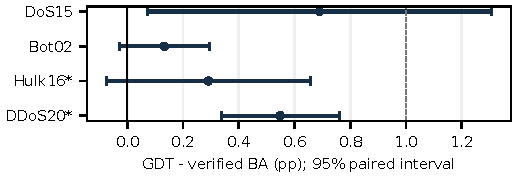
\includegraphics[width=\columnwidth]{figures/paper_gate_increment.pdf}
\caption{Gate-path BA differences versus verified-only, with five-seed paired 95\% intervals. Asterisks mark new captures; the dashed line is the one-point target.}
\label{fig:learning}
\end{figure}

Primary confirmation uses 12,000 DoS flows with 81 attacks (59 GoldenEye, 22 Slowloris) and 12,000 Botnet flows with 334 attacks, sampled chronologically without label selection. A case-control Web challenge contains 12,000 benign flows and 158 attacks (73 XSS, 62 brute force, 23 SQL); a label-blind Web sample with one attack is descriptive only. Duplicate/conflicting fingerprints and historical overlap were removed. Retention probe S3 contains 1,024 balanced flows per seed, session/fingerprint-disjoint from used source data. Its replacement of the smoke-test probe before confirmation is recorded as an amendment. The new Hulk16/DDoS20 captures contain 12,000 flows each, with 3,920/843 attacks. Label-blind fingerprint sampling follows chronological ordering, excludes historical/old-cohort overlap, and uses frozen source transforms. Their 63 shared predictor fingerprints and common testbed limit independence; new capture does not mean a new organization.

\subsection{Confirmation and Matched-Feedback Controls}
Seeds 11, 23, 37, 51, and 79 vary sampling/memory; they are not five independent networks. Four conditions are correct feedback with delay 1; delay 80; independently wrong labels with probability 0.10, corrected 400 events after arrival; and ML2 attack proposals forced benign with probability 0.25 under delay 80. The last perturbation is evaluator-injected. Delay starts at the block-end request; all annotations are simulated.

Original confirmation uses six packages; selected controls appear in Table~\ref{tab:results}. Verified-only and simple maximum share requests, labels, ML2 trajectories, detectors, weights, and cadence with GDT; routing and its induced threshold controller differ. The frozen detector fixes ML1 and threshold while ML2 acquisition continues. Full-history uses 8,192 source samples and a 500-flow cadence, comparing packages rather than memory alone. A predecessor completes the six original packages. A 100\%-label reference runs only under delay 1 and is not an optimal bound. Native ARF (River 0.22.0)~\cite{river} uses ten trees and default ADWIN settings. It shares query identities, arrived labels, and audits, but learns each label once at 100-flow boundaries, without HGB's 1/4/8 weights or replay cadence. Corrections restore its source-initial state and replay latest arrived labels in arrival order. Thus, ARF is a package comparison, not equal memory/computation. Three supported cohorts (DoS/Botnet/Web challenge), plus descriptive Web runs, yield
\begin{equation}
 R=3\cdot5\cdot(6\cdot4+1)+5\cdot3=390.\label{eq:runs}
\end{equation}
The 870 original runs were audited. D5 adds 80 native-ARF runs and 40 shared HGB/NN trajectories: 200 new-capture system evaluations plus 40 old-capture ARF evaluations. Shared routing is not independent retraining.

\subsection{Metrics and Statistical Analysis}
BA weights both classes equally; average precision (AP) complements evaluation of rare attacks~\cite{saito}; FPR measures alarm burden. This combination is used because always predicting benign can appear accurate when attacks are rare. AP evaluates score ranking, whereas BA/FPR evaluate decisions at the applied threshold; they can rank methods differently. For class-decision counts $TP,FN,TN,FP$:
\begin{equation}
 \mathrm{BA}=\tfrac12\left(\frac{TP}{TP+FN}+\frac{TN}{TN+FP}\right),\quad L=\frac{4FN+FP}{N}.\label{eq:metrics}
\end{equation}
Package criteria on each primary capture are mean BA gain $\ge2$ points over frozen, source BA loss $\le2$ points, and FPR $\le2\%$. Against verified-only, gate targets are BA gain $\ge1$ point, source BA gap $\ge-2$ points, and FPR gap $\le1$ point. These study criteria do not qualify production use. Gain thresholds distinguish targeted practical benefit from a merely positive difference; retention/FPR limits prevent target gains from being read without their error costs. A 95\% interval uses paired differences $d_s$ averaged over four conditions per seed:
\begin{equation}
 \bar d\pm t_{0.975;4}\frac{s_d}{\sqrt5},\quad s_d^2=\tfrac14\sum_{s=1}^5(d_s-\bar d)^2.\label{eq:ci}
\end{equation}
Intervals are unadjusted and describe algorithmic variation, not network-wide uncertainty. Consistent gate benefit requires the one-point target and a positive lower interval on both new captures. Raw ML1/ML2 use threshold 0.5; systems use their respective controllers.

\section{Experimental Results and Discussion}
\subsection{Model Performance and Source Retention (RQ1)}
Table~\ref{tab:results} separates the classifiers and their combination. GDT improves BA over frozen by 14.74 points on DoS (29.47\% relative; interval [9.65,19.83]) and 44.32 on Botnet (88.65\%; [40.23,48.40]). Final source BA is 99.58\%/99.37\%, changing by +0.37/+0.15 points from initialization. Package criteria are met, but 29.57\% DoS recall is inadequate for general deployment.

Frozen BA is approximately 50\% with near-zero recall: low FPR accompanies failure to recognize attacks. BA/recall must therefore be read alongside FPR. Source retention shows no mean decline on the probe, without establishing prevention of forgetting across all tasks. Raw ML1/ML2 use threshold 0.5; their gaps from GDT also include its threshold controller, not just gating. ML2 estimates local support, not human analyst capability.

\subsection{Incremental Gate Path under Matched Controls (RQ2)}
Gains over verified-only on DoS/Botnet are 0.69 points (1.08\% relative; [0.07,1.31]) and 0.13 (0.14\%; [-0.03,0.29]). Both miss the one-point target. Simple maximum achieves BA higher by 8.97/1.65 points with FPR below 2\%. The gate changes only 1.4 raw decisions per run on average, despite pooled change precision of 100\%/67.86\%. Candidates were not replaced after confirmation.

High change precision is insufficient when few decisions change. Equation~(\ref{eq:tradeoff}) shows the need for enough rescued attacks relative to additional alarms. Gating restricts when ML2 can raise ML1; simple maximum uses that support more broadly. This is consistent with a possible coverage--conservatism tradeoff, but individual conditions have not been ablated. Because maximum FPR also meets the study limit, gate complexity lacks a strong performance justification. Verified-only isolates the gate path together with threshold changes induced by its scores, rather than its effect at a single locked threshold.

\subsection{Additional Captures and Native ARF (RQ1--2)}
On Hulk16/DDoS20, GDT BA is 96.46\%/91.45\%, versus native ARF 89.10\%/78.08\% (Table~\ref{tab:results}). Gate gains over verified-only are 0.29/0.55 points, with intervals [-0.08, 0.66]/[0.34, 0.76]. Gaps against simple maximum are $-0.69$/$-2.07$ points. Consistent incremental gate benefit is not established. ARF weighting/cadence differ; beating ARF cannot substitute for gate attribution. New-capture FPR is 0.25\%/0.15\%; source BA changes by $-0.35$/$+0.34$ points.

On DDoS20, the interval is above zero but entirely below the one-point target; a positive difference is distinct from the specified practical benefit. The Hulk16 interval crosses zero, so even the direction of benefit is not stable across seed variation. Neither satisfies the joint consistency requirement. Gaps from ARF describe package outcomes under shared queries; replay, weights, fitting schedules, and adaptation mechanisms differ, preventing attribution to a single component. Additional captures broaden testing without removing the shared-testbed limitation.

\subsection{Label Cost and Attack-Family Failures (RQ3)}
For 12,000 flows under delay 80, 600 requests yield 476 arrived training labels and 119 audits; ML1 performs 60 regular refits. Fig.~\ref{fig:learning} shows limited gate increments. Retraining remains uneven. Family recall is 88.85\% for Botnet, 17.20\% GoldenEye, 62.73\% Slowloris, 58.63\% Web brute force, 0\% SQL, and 92.47\% XSS. Only Botnet/XSS among these original families meet 70\%.

The 5\% budget counts requests, not training labels alone: audits are separate and some feedback has not arrived. Refitting demonstrates execution of updates, without ensuring enough positive examples or success on subsequent attacks. Recall differences across families show the need to inspect rare attacks alongside capture averages.

Every SQL run receives a correct training label. Mean remaining attacks after the first ML1/ML2 fit using it are 0/2.4; post-fit recall without positives is undefined. With no subsequent SQL attacks after the ML1 fit, overall 0\% recall does not measure the newly trained ML1's capability on that family. It nevertheless remains a detection failure over the observed horizon, rather than evidence of recovery. Four of 20 DoS runs lack a correct positive audit; mean correct positive training count is 11.45. Audits without positives provide limited information for selecting an attack-sensitive threshold. These counts describe opportunity, not single-factor causation.

\subsection{Contextual Comparison with Prior Studies}
SOUL uses at most 20\% labels~\cite{soul}; Jeon--Kim meets its target for 24/28 attack--classifier pairs~\cite{jeon}. Our 5\% queries and 2/6 original families above 70\% recall do not establish superior efficiency. NAFN's 50\% noise setting~\cite{nafn} differs from our corrected 10\% errors. ACORN-IDS reports F1 gains without attack labels~\cite{acorn}; GDT needs positives. Cross-protocol scores cannot rank these methods; the local ARF comparison is explicit.

Fixed acquisition isolates incremental gate benefit; post-fit labels explain learning opportunities. Table~\ref{tab:lit} maps mechanism differences; Table~\ref{tab:results} compares local outcomes. Percentages from different datasets, label costs, and success criteria remain incomparable.

\balance
\subsection{Limitations and Conclusions}
Shared testbeds, repeated fingerprints, and case-control Web sampling limit generalization. Five seeds are not five networks. Source retention does not measure all-task forgetting; capture resets do not establish lifelong learning. Human agreement/production latency are unmeasured; ARF memory/weights differ; ledger/replay storage grows. New tuning requires separate development/confirmation data.

RQ1: the adaptive package improves over frozen detection with source-probe retention. RQ2: gating misses the consistent-benefit target; simple maximum is stronger in mean BA. RQ3: correct labels alone are insufficient; their entry into fitting and remaining attacks limit observation of update benefits. Simulated annotations do not establish improved human performance.

The contribution is auditable integration, matched acquisition, and opportunity analysis. Additional testing does not establish gate superiority. All feedback is simulated.

\subsection{Data and Artifact Availability}
The \href{https://github.com/langss1/verified-feedback-adaptive-ids}{public GitHub repository} provides versioned data/code. Release \texttt{v1.0.0} supplies 50 prepared NPZ files (development/history, retention, original confirmation) and 870 runs/ledgers; \texttt{v1.1.0} adds ten new-capture NPZ files, initial-state caches, and 240 evaluations. Complete raw datasets are not redistributed.

In \texttt{v1.2.0}, \path{docs/REVIEWER_GUIDE.md} links data maps, schemas, and claim--code--result evidence: roles, dimensions, labels, and hashes. Prepared-array replay is supported; raw reconstruction needs documented dependencies. Code is MIT licensed; dataset rights remain with providers.

\begin{thebibliography}{99}
\bibitem{gama} J. Gama et al., ``A survey on concept drift adaptation'', \emph{ACM Comput. Surv.}, vol. 46, no. 4, art. 44, 2014, doi: 10.1145/2523813.
\bibitem{lu} J. Lu et al., ``Learning under Concept Drift: A Review'', \emph{IEEE TKDE}, vol. 31, no. 12, pp. 2346--2363, 2019, doi: 10.1109/TKDE.2018.2876857.
\bibitem{sharaf} I. Sharafaldin, A. H. Lashkari, and A. A. Ghorbani, ``Toward Generating a New Intrusion Detection Dataset and Intrusion Traffic Characterization'', \emph{ICISSP}, pp. 108--116, 2018, doi: 10.5220/0006639801080116.
\bibitem{engelen} G. Engelen, V. Rimmer, and W. Joosen, ``Troubleshooting an Intrusion Detection Dataset: the CICIDS2017 Case Study'', \emph{IEEE SPW/WTMC}, pp. 7--12, 2021, doi: 10.1109/SPW53761.2021.00009.
\bibitem{liu} L. Liu et al., ``Error Prevalence in NIDS datasets: A Case Study on CIC-IDS-2017 and CSE-CIC-IDS-2018'', \emph{IEEE CNS}, 2022.
\bibitem{arp} D. Arp et al., ``Dos and Don'ts of Machine Learning in Computer Security'', \emph{USENIX Security}, pp. 3971--3988, 2022.
\bibitem{tesseract} F. Pendlebury et al., ``TESSERACT: Eliminating Experimental Bias in Malware Classification across Space and Time'', \emph{USENIX Security}, pp. 729--746, 2019.
\bibitem{paired} S. H. Bach and M. A. Maloof, ``Paired Learners for Concept Drift'', \emph{IEEE ICDM}, pp. 23--32, 2008.
\bibitem{sam} V. Losing, B. Hammer, and H. Wersing, ``Self-Adjusting Memory: How to Deal with Diverse Drift Types'', \emph{IJCAI}, pp. 4899--4903, 2017, doi: 10.24963/ijcai.2017/690.
\bibitem{adwin} A. Bifet and R. Gavalda, ``Learning from Time-Changing Data with Adaptive Windowing'', \emph{SIAM SDM}, pp. 443--448, 2007, doi: 10.1137/1.9781611972771.42.
\bibitem{arf} H. M. Gomes et al., ``Adaptive random forests for evolving data stream classification'', \emph{Mach. Learn.}, vol. 106, pp. 1469--1495, 2017, doi: 10.1007/s10994-017-5642-8.
\bibitem{soul} S. K. Amalapuram et al., ``SOUL: A Semi-supervised Open-world continUal Learning method for Network Intrusion Detection'', \emph{arXiv:2412.00911}, 2024.
\bibitem{ssf} X. Zhang et al., ``Continual Learning with Strategic Selection and Forgetting for Network Intrusion Detection'', \emph{IEEE INFOCOM}, arXiv:2412.16264v4, 2025.
\bibitem{jeon} S. Jeon and A. Kim, ``A Label-Efficient Adaptive Retraining Framework for Network Intrusion Detection Under Streaming Arrival Bias'', \emph{Electronics}, vol. 15, no. 17, art. 3812, 2026, doi: 10.3390/electronics15173812.
\bibitem{nafn} Z. Zhao et al., ``Network Intrusion Detection Adaptability under Spurious Labels: A Noise-Aware Few-Shot Class-Incremental Learning Framework'', \emph{IEEE TNSM}, 2026, doi: 10.1109/TNSM.2026.3752751.
\bibitem{acorn} S. Fuhrman, O. Gungor, and T. Rosing, ``ACORN-IDS: Adaptive Continual Novelty Detection for Intrusion Detection Systems'', \emph{arXiv:2602.07291}, 2026.
\bibitem{friedman} J. H. Friedman, ``Greedy function approximation: A gradient boosting machine'', \emph{Ann. Statist.}, vol. 29, no. 5, pp. 1189--1232, 2001, doi: 10.1214/aos/1013203451.
\bibitem{lightgbm} G. Ke et al., ``LightGBM: A Highly Efficient Gradient Boosting Decision Tree'', \emph{NeurIPS}, vol. 30, pp. 3146--3154, 2017.
\bibitem{sklearn} scikit-learn developers, ``Histogram-Based Gradient Boosting'', \emph{scikit-learn 1.9.1 documentation}, accessed Nov. 26, 2026, \url{https://scikit-learn.org/stable/modules/ensemble.html}.
\bibitem{cover} T. Cover and P. Hart, ``Nearest neighbor pattern classification'', \emph{IEEE Trans. Inf. Theory}, vol. 13, no. 1, pp. 21--27, 1967, doi: 10.1109/TIT.1967.1053964.
\bibitem{dudani} S. A. Dudani, ``The Distance-Weighted k-Nearest-Neighbor Rule'', \emph{IEEE Trans. Syst., Man, Cybern.}, vol. SMC-6, no. 4, pp. 325--327, 1976, doi: 10.1109/TSMC.1976.5408784.
\bibitem{guo} C. Guo et al., ``On Calibration of Modern Neural Networks'', \emph{ICML/PMLR}, vol. 70, pp. 1321--1330, 2017.
\bibitem{settles} B. Settles, ``Active Learning Literature Survey'', \emph{Univ. Wisconsin--Madison}, Tech. Rep. 1648, revised Jan. 2010, 2009.
\bibitem{tavallaee} M. Tavallaee et al., ``A Detailed Analysis of the KDD CUP 99 Data Set'', \emph{IEEE CISDA}, pp. 1--6, 2009, doi: 10.1109/CISDA.2009.5356528.
\bibitem{moustafa} N. Moustafa and J. Slay, ``UNSW-NB15: a comprehensive data set for network intrusion detection systems (UNSW-NB15 network data set)'', \emph{IEEE MilCIS}, pp. 1--6, 2015, doi: 10.1109/MilCIS.2015.7348942.
\bibitem{river} River developers, ``ARFClassifier'', \emph{River 0.22.0 documentation}, accessed Nov. 26, 2026, \url{https://riverml.xyz/0.22.0/api/forest/ARFClassifier/}.
\bibitem{saito} T. Saito and M. Rehmsmeier, ``The Precision-Recall Plot Is More Informative than the ROC Plot When Evaluating Binary Classifiers on Imbalanced Datasets'', \emph{PLoS ONE}, vol. 10, no. 3, e0118432, 2015, doi: 10.1371/journal.pone.0118432.
\end{thebibliography}
\end{document}
